\documentclass[tikz,border=4pt]{standalone}
\usepackage{tikz}
\usetikzlibrary{arrows.meta,calc,decorations.pathmorphing,positioning}
\definecolor{electrode}{HTML}{34495E}
\definecolor{film}{HTML}{F4E5A5}
\definecolor{trap}{HTML}{A53B3B}
\definecolor{signal}{HTML}{2D6F8E}
\definecolor{ink}{HTML}{222222}
\tikzset{
  every node/.style={font=\sffamily\scriptsize,text=ink},
  panel/.style={font=\sffamily\bfseries\small,text=ink},
  electrode/.style={fill=electrode,draw=none},
  film/.style={fill=film,draw=ink!55,line width=.35pt},
  trapsite/.style={text=trap,font=\sffamily\normalsize},
  transport/.style={draw=signal,line width=.8pt,-{Stealth[length=2.4mm]},rounded corners=1.3pt},
  insetaxis/.style={draw=ink!70,line width=.35pt},
  dist/.style={draw=signal!85!black,fill=signal!18,line width=.65pt},
  measure/.style={draw=trap,line width=.5pt,{Stealth[length=1.8mm]}-{Stealth[length=1.8mm]}}
}
\begin{document}
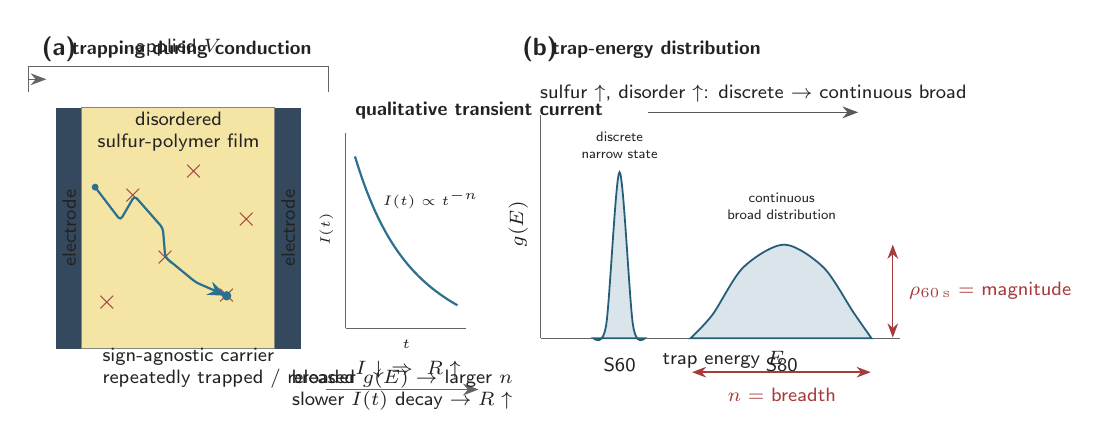
\begin{tikzpicture}[x=1cm,y=1cm]
  % Panel A: applied-bias cell, repeated sign-neutral trapping, and decay inset.
  \node[panel,anchor=west] at (0,4.52) {(a)};
  \node[anchor=west,font=\sffamily\bfseries\scriptsize] at (.38,4.52)
    {trapping during conduction};
  \draw[electrode] (.30,.72) rectangle (.63,3.78);
  \draw[electrode] (3.08,.72) rectangle (3.41,3.78);
  \draw[film] (.63,.72) rectangle (3.08,3.78);
  \node[rotate=90,font=\sffamily\scriptsize] at (.47,2.25) {electrode};
  \node[rotate=90,font=\sffamily\scriptsize] at (3.25,2.25) {electrode};
  \node[align=center,font=\sffamily\scriptsize] at (1.86,3.48) {disordered\\sulfur-polymer film};
  \foreach \x/\y in {.95/1.30,1.28/2.66,1.69/1.88,2.05/2.97,2.47/1.39,2.72/2.36}
    \node[trapsite] at (\x,\y) {$\times$};
  \draw[transport] (.80,2.77) -- (1.12,2.35) -- (1.30,2.66) -- (1.66,2.25)
    -- (1.69,1.88) -- (2.08,1.56) -- (2.47,1.39);
  \fill[signal] (.80,2.77) circle (1.25pt);
  \fill[signal] (2.47,1.39) circle (1.7pt);
  \node[anchor=west,align=left] at (.77,.47) {sign-agnostic carrier\\repeatedly trapped / released};
  \draw[draw=ink!70,line width=.35pt] (-.05,3.98) -- (-.05,4.30) -- (3.76,4.30) -- (3.76,3.98);
  \draw[-{Stealth[length=2mm]},draw=ink!70,line width=.4pt] (-.05,4.14) -- (.18,4.14);
  \node[anchor=south,font=\sffamily\scriptsize] at (1.86,4.31) {applied $V$};

  \begin{scope}[shift={(3.98,.98)}]
    \node[anchor=west,font=\sffamily\scriptsize\bfseries] at (0,2.76) {qualitative transient current};
    \draw[insetaxis] (0,0) -- (0,2.48);
    \draw[insetaxis] (0,0) -- (1.53,0);
    \node[anchor=north,font=\sffamily\tiny] at (.77,-.03) {$t$};
    \node[anchor=south,rotate=90,font=\sffamily\tiny] at (-.03,1.25) {$I(t)$};
    \draw[signal,line width=.8pt] (.12,2.18) .. controls (.43,1.15) and (.82,.63) .. (1.42,.29);
    \node[anchor=west,font=\sffamily\tiny] at (.35,1.63) {$I(t)\propto t^{-n}$};
    \node[align=left,anchor=west,font=\sffamily\scriptsize] at (0,-.53)
      {$I\downarrow\ \Rightarrow\ R\uparrow$};
  \end{scope}

  % Panel B: distribution form, width n, and independent magnitude rho_60s.
  \begin{scope}[shift={(6.10,0)}]
    \node[panel,anchor=west] at (0,4.52) {(b)};
    \node[anchor=west,font=\sffamily\bfseries\scriptsize] at (.38,4.52)
      {trap-energy distribution};
    \draw[insetaxis] (.36,.85) -- (.36,3.68);
    \draw[insetaxis] (.36,.85) -- (4.92,.85);
    \node[anchor=north,font=\sffamily\scriptsize] at (2.68,.81) {trap energy $E$};
    \node[anchor=south,rotate=90,font=\sffamily\scriptsize] at (.32,2.30) {$g(E)$};
    % A narrow, discrete S60 state.
    \draw[dist] plot[smooth] coordinates {(1.03,.85) (1.19,1.02) (1.36,2.96) (1.53,1.02) (1.68,.85)} -- cycle;
    \node[anchor=north,font=\sffamily\scriptsize] at (1.36,.73) {S60};
    \node[align=center,font=\sffamily\tiny] at (1.36,3.30) {discrete\\narrow state};
    % A broad, continuous S80 distribution.
    \draw[dist] plot[smooth] coordinates {(2.26,.85) (2.54,1.15) (2.93,1.75) (3.45,2.04) (3.95,1.75) (4.33,1.18) (4.56,.85)} -- cycle;
    \node[anchor=north,font=\sffamily\scriptsize] at (3.42,.73) {S80};
    \node[align=center,font=\sffamily\tiny] at (3.42,2.53) {continuous\\broad distribution};
    % Width and amplitude are explicitly orthogonal measurements.
    \draw[measure] (2.28,.42) -- (4.55,.42);
    \node[anchor=north,text=trap,font=\sffamily\scriptsize] at (3.42,.34) {$n$ = breadth};
    \draw[measure] (4.83,.86) -- (4.83,2.04);
    \node[anchor=west,text=trap,font=\sffamily\scriptsize] at (4.91,1.46) {$\rho_{60\,\mathrm{s}}$ = magnitude};
    \draw[-{Stealth[length=2mm]},draw=ink!75,line width=.45pt] (1.72,3.72) -- (4.39,3.72);
    \node[anchor=south,font=\sffamily\scriptsize] at (3.06,3.73)
      {sulfur $\uparrow$, disorder $\uparrow$: discrete $\rightarrow$ continuous broad};
  \end{scope}

  % One uncluttered causal bridge across the two schematic blocks.
  \draw[-{Stealth[length=2mm]},draw=ink!70,line width=.45pt] (3.73,.20) -- (5.67,.20);
  \node[align=center,font=\sffamily\scriptsize] at (4.70,.20)
    {broader $g(E)$ $\rightarrow$ larger $n$\\slower $I(t)$ decay $\rightarrow R\uparrow$};
\end{tikzpicture}
\end{document}
